\section{Results}

\subsection{Best Observed Performance Across the Full Grid}

Table~\ref{tab:best_models} reports the best observed performance per endpoint across all 
225 configurations. These values are an upper bound from extensive search and should be read 
as a descriptive benchmark, not unbiased estimates; the confirmatory analysis uses the fixed 
configuration (Table~\ref{tab:cascade}).

\begin{table}[ht]
\caption{Best observed performance per endpoint (scaffold-split test set, full grid). Best 
among 225 configurations; descriptive benchmark, not unbiased estimates.}
\label{tab:best_models}
\centering
\small
\begin{tabular}{@{}llllccccc@{}}
\toprule
Endpoint & Algo. & Preproc. & Features ($n$) & MCC [95\% CI] & AUC & PR-AUC & Sens. & Spec. \\
\midrule
Ames     & XGB  & raw      & FP-2048 (522) & 0.555 [.522,.588]    & 0.850 & 0.765 & 0.756 & 0.822 \\
In vitro & LGBM & salt\_str. & FP-1024 (394) & 0.297 [.131,.450]  & 0.665 & 0.278 & 0.349 & 0.929 \\
In vivo  & XGB  & salt\_str. & FP-512 (266)  & 0.311 [$-$.014,.571] & 0.860 & 0.237 & 0.319 & 0.983 \\
\bottomrule
\end{tabular}

\medskip
\footnotesize
PR-AUC baselines (prevalence): Ames 0.302, \textit{in vitro} 0.124, \textit{in vivo} 0.028.
\end{table}

Under fixed features and preprocessing (compact, raw SMILES), all seven algorithms on Ames 
spanned an MCC range of only 0.063 (Table~\ref{tab:all_algorithms}, 
Figure~\ref{fig:model_comparison}); the five tabular models excluding LR spanned 0.023. 
Pairwise McNemar tests\cite{McNemar_1947} between the top two models found no significant 
differences (Ames $p = 0.39$; \textit{in vivo} $p = 0.72$). This in-domain equivalence did not 
extend to cross-source settings (see \textit{Data Source Heterogeneity and Algorithm-Specific Robustness}).

The GCN underperformed 
fingerprint-based approaches across endpoints (Ames mean MCC 0.402 vs.\ 0.507 for XGB), 
consistent with prior reports that graph networks require considerably larger datasets to 
outperform engineered features.

\begin{table}[ht]
\caption{All-algorithm comparison (compact features, raw SMILES, Ames scaffold-split test). 
Range across all 7 algorithms: 0.063; range excluding LR and GCN: 0.023.}
\label{tab:all_algorithms}
\centering
\small
\begin{tabular}{@{}lcc@{}}
\toprule
Algorithm & MCC & ROC-AUC \\
\midrule
RF       & 0.492 & 0.838 \\
ANN (MLP) & 0.489 & 0.834 \\
LGBM     & 0.479 & 0.833 \\
SVM (RBF) & 0.470 & 0.832 \\
XGB      & 0.470 & 0.825 \\
GCN      & 0.445 & 0.815 \\
LR       & 0.430 & 0.800 \\
\bottomrule
\end{tabular}
\end{table}

\begin{figure}[ht]
\centering
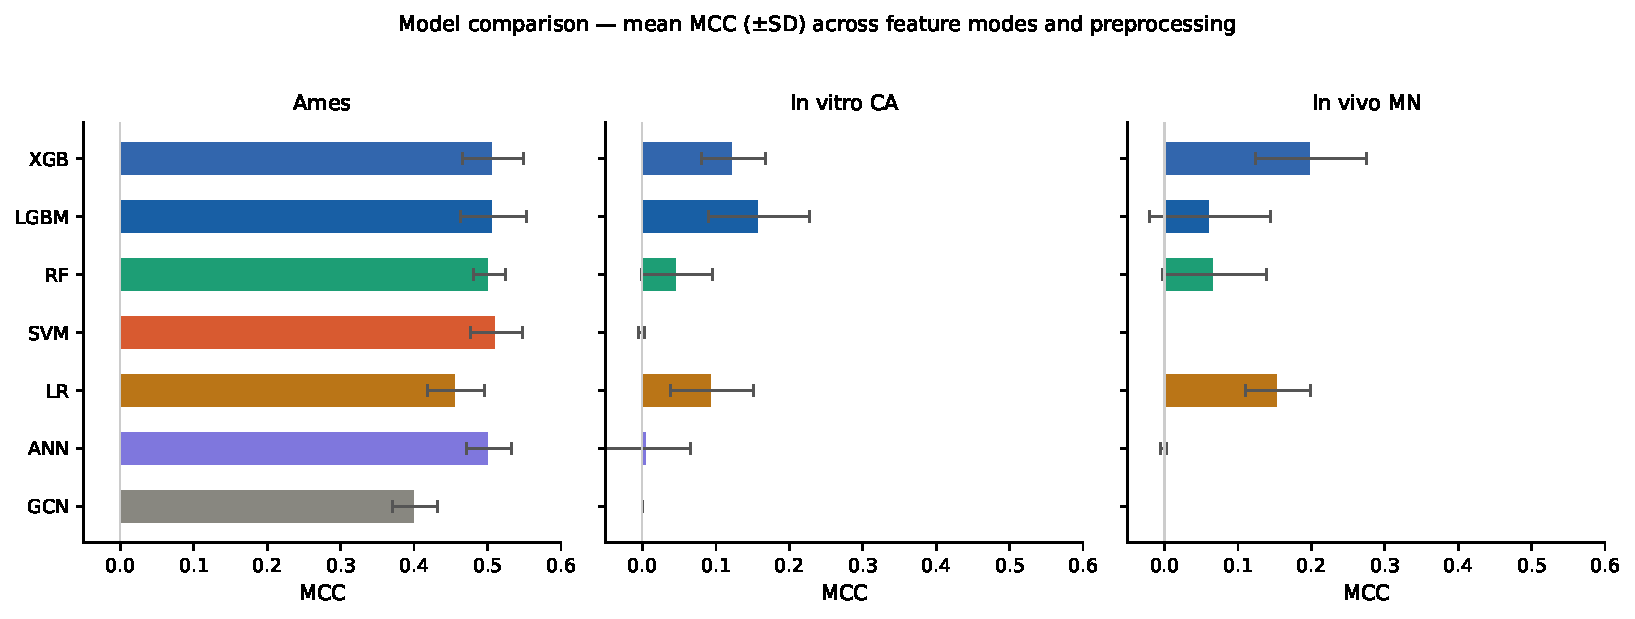
\includegraphics[width=\textwidth]{figures/figure2_model_comparison.pdf}
\caption{Mean MCC ($\pm$SD) by algorithm across all feature modes and preprocessing 
scenarios, grouped by endpoint.}
\label{fig:model_comparison}
\end{figure}

\subsection{Evaluation Cascade}

For Ames, random-split CV reached MCC = $0.670 \pm 0.010$, in line with published 
benchmarks,\cite{Hansen_2009,Li_2021} while scaffold-split CV fell to $0.624 \pm 0.049$ 
($\Delta = 0.046$) and the held-out scaffold-based test set to 0.470 
(Table~\ref{tab:cascade}, Figure~\ref{fig:cascade}). Cross-source LDO revealed a 
markedly larger decline: drug$\to$industrial yielded MCC = 0.234 and 
industrial$\to$drug yielded MCC = 0.122. The source heterogeneity gap ($\Delta = 0.390$) 
was considerably larger than the split-method gap ($\Delta = 0.046$). The LDO values also 
reflect differences in test set size and class distribution across directions, so 
$\Delta = 0.390$ captures a combined effect rather than source heterogeneity alone---but 
the relative magnitude of the two effects is unambiguous. For \textit{in vitro} CA, random and 
scaffold splits yielded nearly identical results (0.180 vs.\ 0.189); for \textit{in vivo} MN, both 
values were near chance level given their standard deviations.

\begin{table}[ht]
\caption{Evaluation cascade (fixed configuration: XGBoost, compact features, raw SMILES). 
Level 2: mean $\pm$ SD (25 folds). Level 1: MCC [95\% bootstrap CI]. Level 3: Ames only.}
\label{tab:cascade}
\centering
\small
\begin{tabular}{@{}llccc@{}}
\toprule
Level & Evaluation method & Ames MCC & In vitro MCC & In vivo MCC \\
\midrule
2a & Random-split $5\!\times\!5$ CV    & $0.670 \pm 0.010$ & $0.180 \pm 0.053$ & $0.181 \pm 0.094$ \\
2b & Scaffold-split $5\!\times\!5$ CV  & $0.624 \pm 0.049$ & $0.189 \pm 0.084$ & $0.104 \pm 0.111$ \\
1  & Scaffold-split test               & 0.470 [.434,.502] & 0.114 [$-$.023,.270] & 0.071 [$-$.029,.285] \\
3a & LDO: drug $\to$ industrial        & 0.234 & --- & --- \\
3b & LDO: industrial $\to$ drug        & 0.122 & --- & --- \\
\bottomrule
\end{tabular}
\end{table}

\begin{figure}[ht]
\centering
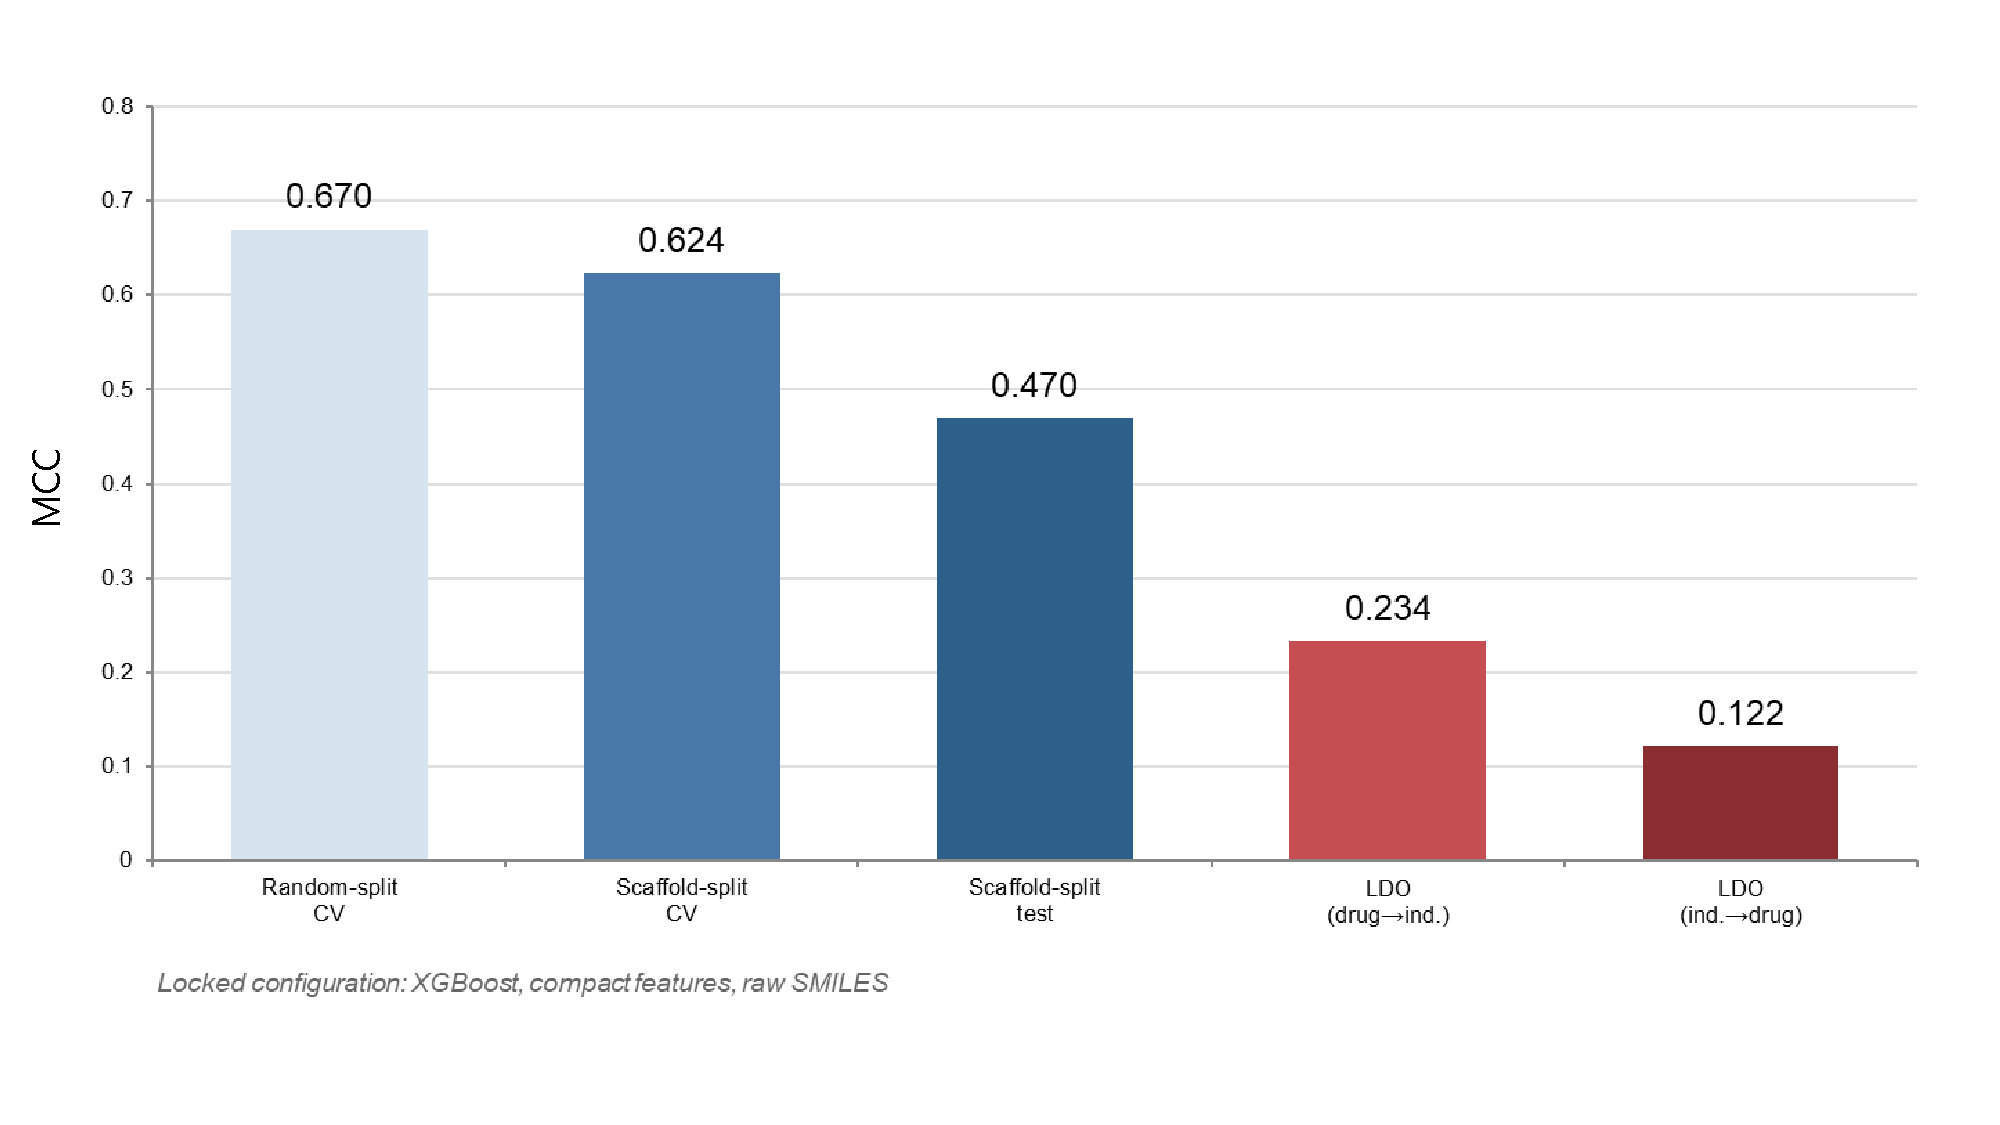
\includegraphics[width=0.85\textwidth]{figures/figure3_cascade.pdf}
\caption{Evaluation cascade for Ames mutagenicity (fixed configuration). The data source 
heterogeneity effect ($\Delta = 0.390$) clearly exceeds the split-method effect 
($\Delta = 0.046$).}
\label{fig:cascade}
\end{figure}

\subsection{Data Source Heterogeneity and Algorithm-Specific Robustness}
\label{sec:domain}

Drug-sourced compounds ($n = 6{,}416$, positive rate 58.3\%) and industrial-sourced 
compounds ($n = 7{,}144$, positive rate 3.0\%) differed by a factor of 19.5 in 
mutagenicity prevalence (Figure~\ref{fig:domain}). A naive classifier predicting positive 
for drug-sourced and negative for industrial-sourced compounds achieved MCC = 0.608 and 
balanced accuracy = 0.834 without any structural information---approaching the random-split 
CV MCC of 0.670.

Comparing three algorithms under LDO (Table~\ref{tab:ldo}) revealed two distinct patterns. 
Drug$\to$industrial generalization was consistent across all algorithms (MCC 0.232--0.235). 
The industrial$\to$drug direction exposed sharp differences: XGB reached only MCC = 0.122 
(sensitivity 0.062) and LGBM 0.134, while RF maintained MCC = 0.325 (sensitivity 0.466). We hypothesize 
that RF's better cross-source robustness may reflect random feature subsampling at each 
split (random subspace method),\cite{Breiman_2001} which reduces reliance on 
source-correlated feature subsets.

\begin{table}[ht]
\caption{Leave-domain-out results by algorithm (Ames). Drug: $n = 6{,}416$, pos.\ rate 
58.3\%. Industrial: $n = 7{,}144$, pos.\ rate 3.0\%. Naive source classifier: MCC = 0.608.}
\label{tab:ldo}
\centering
\small
\begin{tabular}{@{}lccc@{}}
\toprule
Algorithm & Drug $\to$ Ind.\ MCC & Ind.\ $\to$ Drug MCC & Ind.\ $\to$ Drug Sens. \\
\midrule
XGB  & 0.234 & 0.122 & 0.062 \\
LGBM & 0.232 & 0.134 & 0.081 \\
RF   & 0.235 & 0.325 & 0.466 \\
\bottomrule
\end{tabular}
\end{table}

\begin{figure}[ht]
\centering
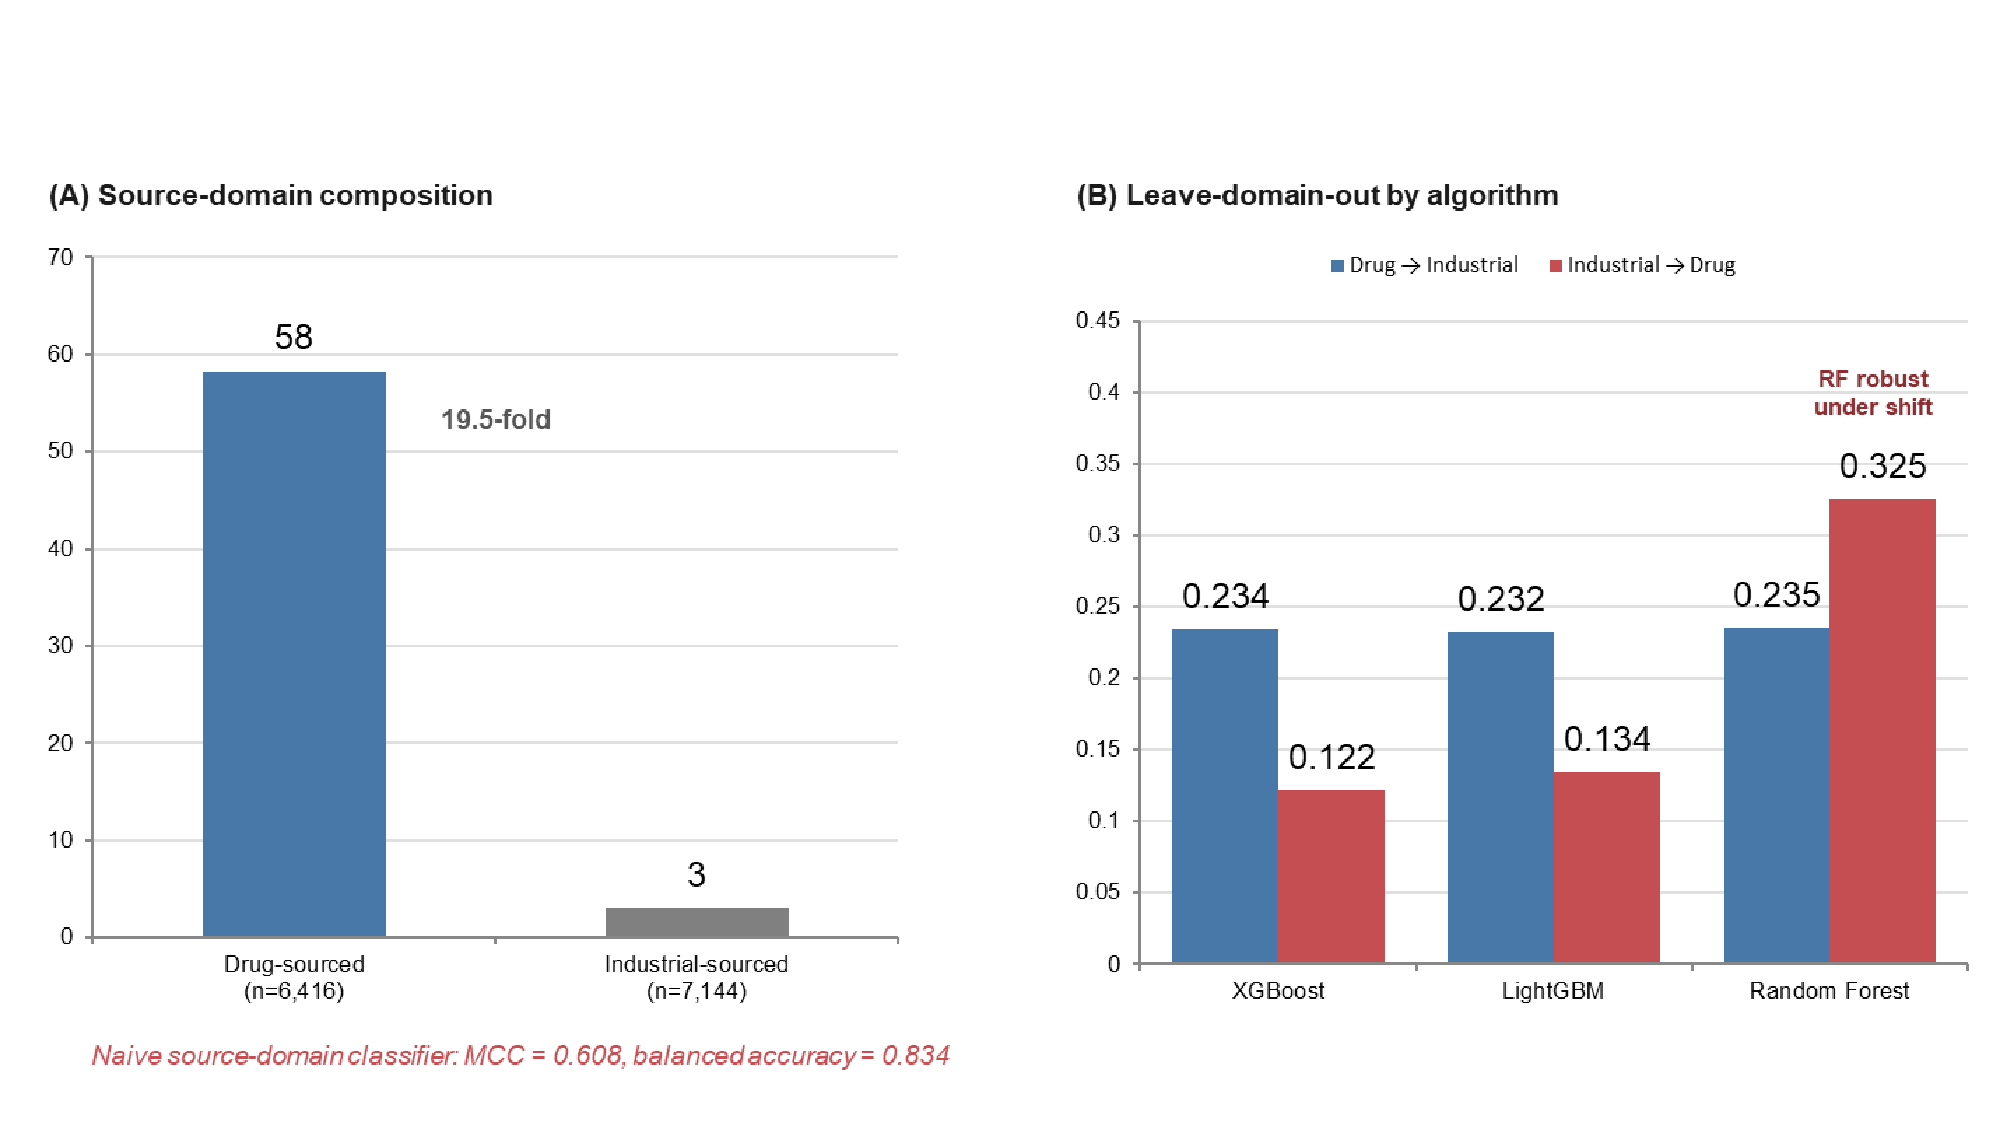
\includegraphics[width=\textwidth]{figures/figure4_domain_ldo.pdf}
\caption{Data source heterogeneity in Ames. (A)~Positive rate by source: drug 58.3\% vs.\ 
industrial 3.0\% (19.5-fold). (B)~LDO MCC by algorithm; RF was appreciably more robust in 
the industrial$\to$drug direction.}
\label{fig:domain}
\end{figure}

\subsection{Preprocessing, \textit{In Vivo} Behavior, and Feature Importance}

\textbf{Preprocessing.} Salt stripping effects were strongly endpoint-specific 
(Figure~\ref{fig:salt}). For \textit{in vivo} MN, the best salt-stripped model reached MCC = 0.311 
versus 0.086 for the best raw model ($+0.225$). Salt fragments were present in 83\% of 
\textit{in vivo} SMILES. Among salt-containing compounds, the positive rate was 2.8\% versus 7.1\% 
for non-salt compounds, indicating that salts were disproportionately associated with 
non-mutagenic structures. For Ames, salt stripping had mixed effects ($\Delta = -0.03$ to 
$+0.02$). For \textit{in vitro} CA it was generally detrimental (mean MCC $0.081 \to 0.056$). These 
results argue against uniform preprocessing across endpoints and support endpoint-specific 
optimization.

\begin{figure}[ht]
\centering
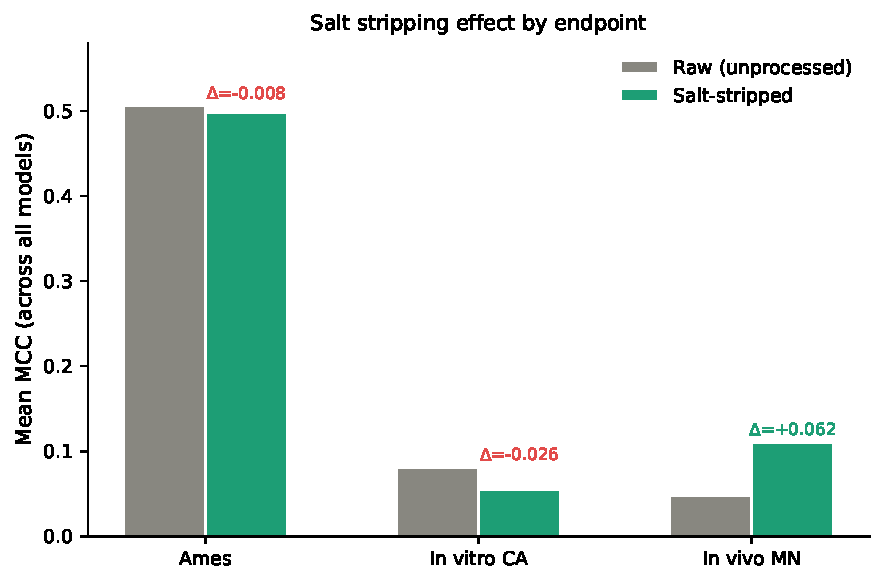
\includegraphics[width=0.75\textwidth]{figures/figure5_salt_stripping.pdf}
\caption{Effect of salt stripping on mean MCC (averaged across all models and feature 
modes). \textit{In vivo} improved by $+0.063$ on average and $+0.225$ for the best model; Ames 
mixed; \textit{in vitro} decreased.}
\label{fig:salt}
\end{figure}

\textbf{\textit{In vivo} micronucleus.} The best \textit{in vivo} model achieved ROC-AUC = 0.860 and PR-AUC 
= 0.237 (an 8.5-fold enrichment over the 0.028 baseline), but MCC = 0.311 with a 95\% CI 
that crossed zero ($-0.014$ to 0.571), meaning classification at any fixed threshold is 
unreliable. The test set contains only 12 positives among 431 compounds. The 
fixed-configuration learning curve was flat at MCC $\approx 0.055$ from 10\% to 100\% of 
training data (Figure~\ref{fig:learning_curves}), though this curve was not computed for the 
salt-stripped configuration.

\textbf{Feature importance.} SHAP analysis\cite{Lundberg_SHAP_2017} revealed consistent 
patterns (Figure~\ref{fig:shap}). Physicochemical descriptors dominated the top-5 at every 
endpoint (alert count and MW for Ames; LogP for \textit{in vitro}; MW for \textit{in vivo}). No individual 
fingerprint bit appeared in any top-5 list, despite fingerprints comprising 50--75\% of 
features. Across all Ames configurations, compact features yielded mean MCC = 0.448 versus 
0.523 for FP-2048 ($\Delta = +0.075$), indicating that fingerprint bits contribute weak 
signal individually but accumulate meaningful predictive information collectively.

\begin{figure}[ht]
\centering
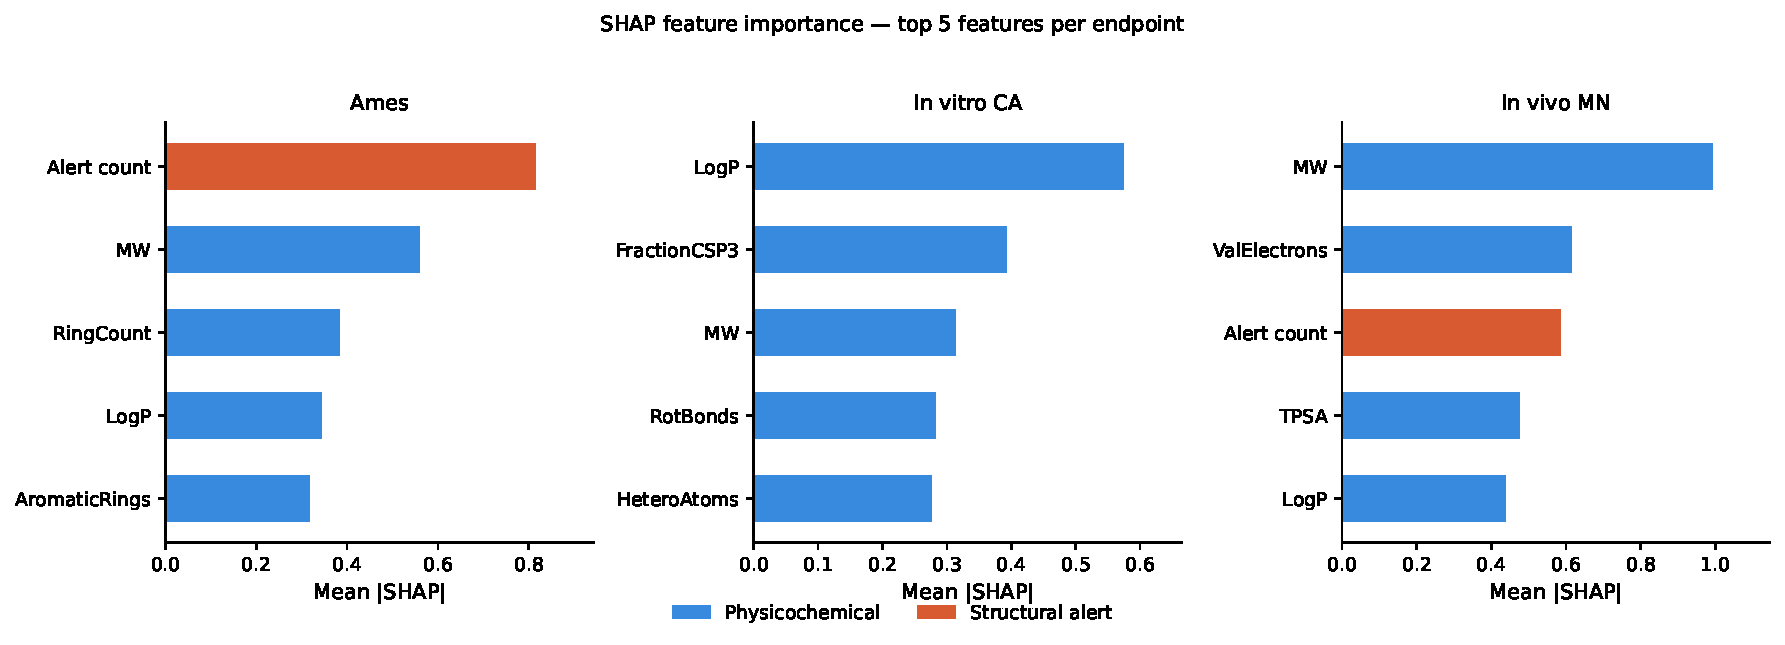
\includegraphics[width=\textwidth]{figures/figure6_shap.pdf}
\caption{SHAP top-5 features per primary endpoint. Physicochemical descriptors dominate; 
structural alert count ranks first for Ames. No fingerprint bits appear in any top-5.}
\label{fig:shap}
\end{figure}

\textbf{Learning curves.} Fixed-configuration learning curves (Figure~\ref{fig:learning_curves}) 
showed three patterns: Ames MCC saturated early (0.543 at 10\%, 0.640 at 100\%); \textit{in vitro} 
showed a noisy upward trend ($0.070 \to 0.170$); \textit{in vivo} remained flat ($\approx 0.055$).

\begin{figure}[ht]
\centering
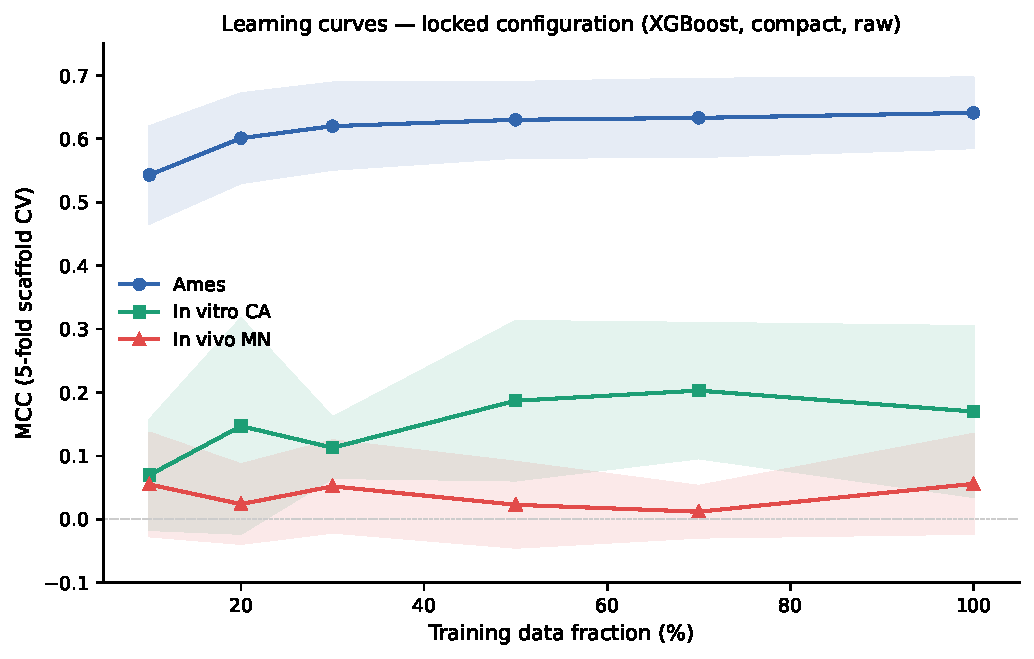
\includegraphics[width=0.8\textwidth]{figures/figure7_learning_curves.pdf}
\caption{Learning curves (fixed configuration). Shaded regions: $\pm$1 SD across 5-fold 
scaffold CV.}
\label{fig:learning_curves}
\end{figure}
